% -----------------------------------------------------------------
% 2. WBS Dictionary
% -----------------------------------------------------------------
\section{WBS Dictionary}

\subsection{Datos Generales}

\begin{tabularx}{\textwidth}{@{}lX@{}}
\textbf{Project Title:} & Hub Financiero \\
\textbf{Date Prepared:} & 21/08/2025 \\
\end{tabularx}

\subsection{Relación con el EDT}

La información de este diccionario corresponde a los paquetes de trabajo \textbf{1.5.1 Mobiliario} y \textbf{1.5.2 Tecnología} del EDT del proyecto (véase la Figura~\ref{fig:edt}).

\begin{figure}[H]
  \centering
  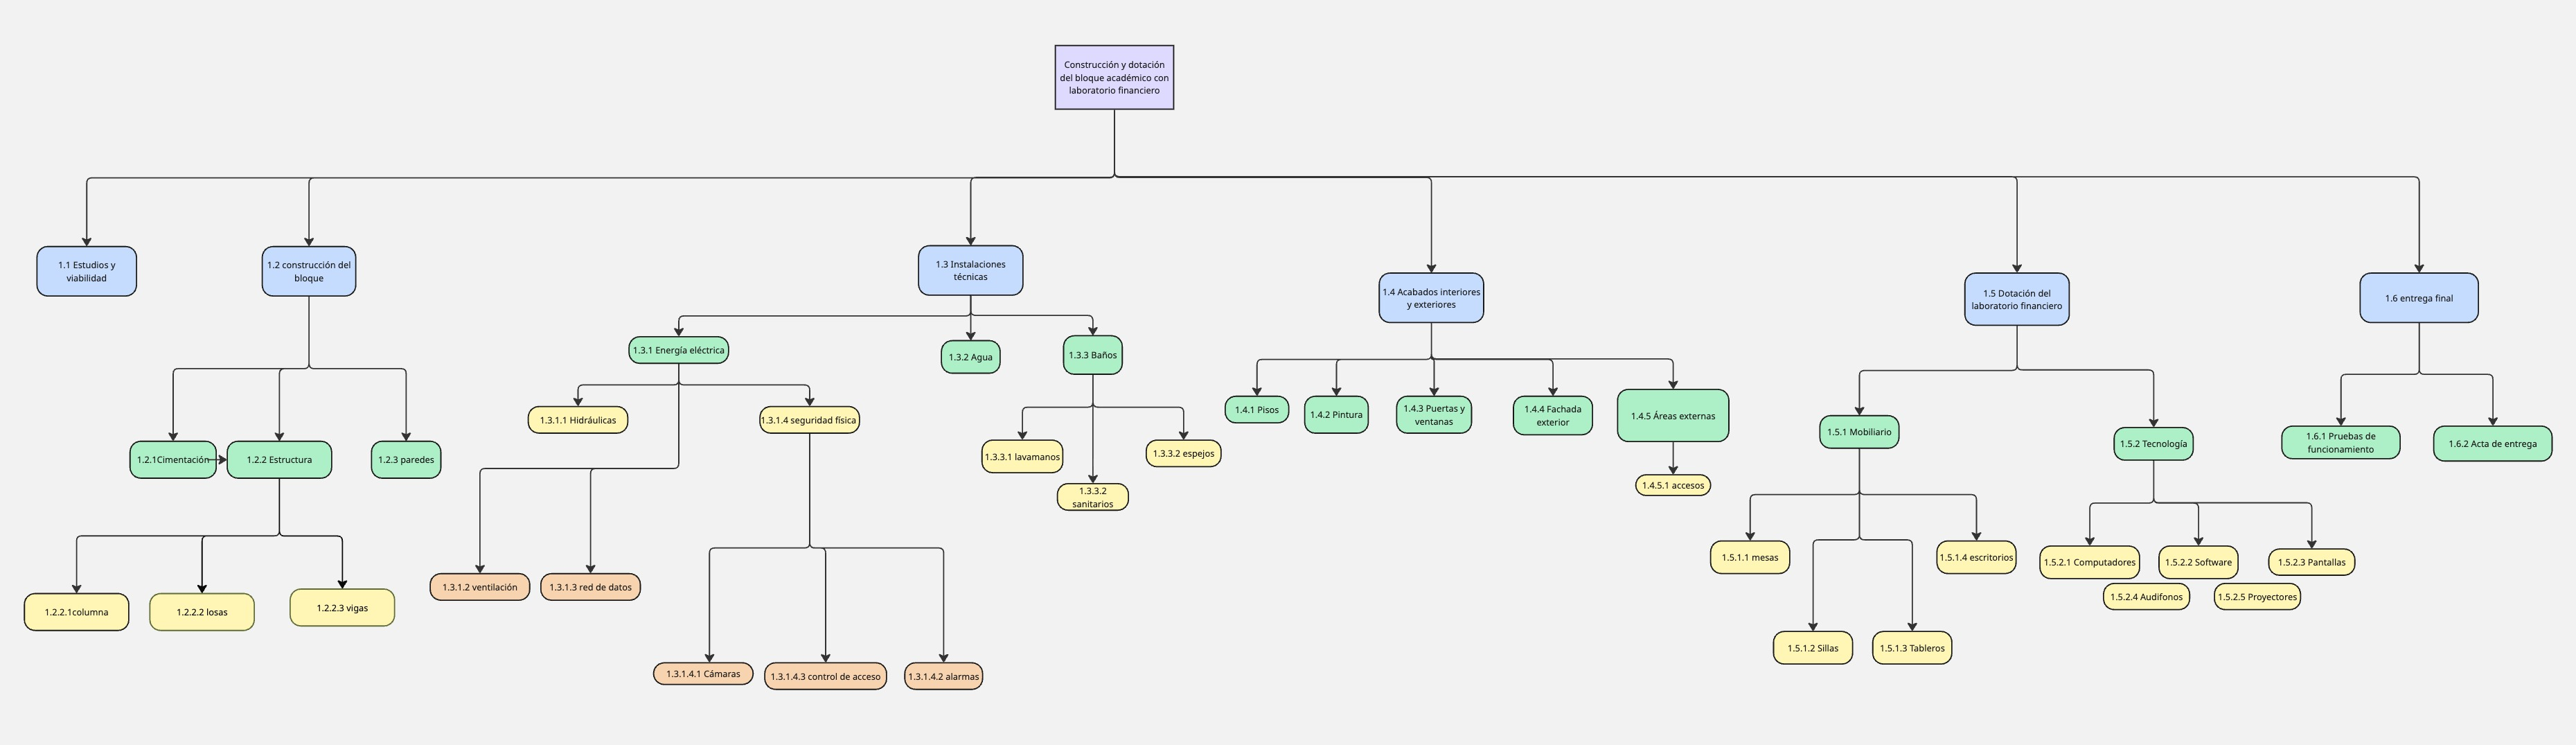
\includegraphics[width=\textwidth]{Figures/0. General/EDT.jpg}
  \caption{Estructura de Desglose del Trabajo (EDT) del proyecto.}
  \label{fig:edt}
\end{figure}

% ================================================================
% PAQUETE 1.5.1 MOBILIARIO
% ================================================================
\subsection{Paquete de Trabajo 1.5.1: Mobiliario}
\label{sec:wbs151}

\begin{tabularx}{\textwidth}{@{}lX@{}}
\textbf{Work Package Name:} & 1.5.1 Mobiliario \\
\textbf{Code of Accounts:} & 1.5.1 \\
\end{tabularx}

\subsubsection*{Descripción}
Dotación de mobiliario del laboratorio financiero, incluyendo mesas, sillas, tableros y escritorios, garantizando espacios adecuados, ergonómicos y estéticos para el aprendizaje.

\subsubsection*{Supuestos y Restricciones}
\begin{itemize}
    \item Entrega e instalación en sitio con supervisión de la Universidad.
    \item Precios dentro de rangos pactados en cotizaciones/contratos.
    \item Cumplimiento de estándares de ergonomía y resistencia aprobados por la Universidad.
\end{itemize}

\subsubsection*{Actividades y Detalles}

\begin{longtable}{|>{\raggedright\arraybackslash}p{1.2cm}|
                        >{\raggedright\arraybackslash}p{1.8cm}|
                        >{\raggedright\arraybackslash}p{2.2cm}|
                        >{\raggedright\arraybackslash}p{2.8cm}|
                        >{\raggedright\arraybackslash}p{2.2cm}|
                        >{\raggedright\arraybackslash}p{4.4cm}|}
\hline
\textbf{WBS ID} & \textbf{Elemento} & \textbf{Proveedor} & \textbf{Costo Unitario (COP)} & \textbf{Fecha Entrega} & \parbox{5.0cm}{\centering\textbf{Criterio de Aceptación}} \\
\hline
\endfirsthead
\hline
\textbf{WBS ID} & \textbf{Elemento} & \textbf{Proveedor} & \textbf{Costo Unitario (COP)} & \textbf{Fecha Entrega} & \parbox{5.0cm}{\centering\textbf{Criterio de Aceptación}} \\
\hline
\endhead
1.5.1.1 & Mesas & Mesas y Sillas Medellín SAS &
900,000 -- 1,600,000 & 10 Nov 2026 &
Mesas blancas hechas a la medida, con instalación por el productor. Entrega en la fecha pactada y verificación de nivelación/estabilidad. \\
\hline
1.5.1.2 & Sillas & Mesas y Sillas Medellín SAS &
250,000 -- 400,000 & 12 Nov 2026 &
Sillas ergonómicas color negro, ensambladas e instaladas en salones. Revisión de ergonomía y ausencia de defectos. \\
\hline
1.5.1.3 & Tableros & Todo Acrílico SAS &
300,000 -- 800,000 & 13 Nov 2026 &
Tableros acrílicos instalados en pared o soporte, superficie limpia y lista para uso en presentaciones/simulaciones. \\
\hline
1.5.1.4 & Escritorios & Scribtorios SAS &
250,000 -- 500,000 & 15 Nov 2026 &
Escritorios individuales con silla incorporada. Precio negociado 250,000 según contrato. Instalación completa en aulas. \\
\hline
\end{longtable}

\subsubsection*{Requisitos de Calidad}
\begin{itemize}
    \item Cumplimiento de normas de seguridad y ergonomía.
    \item Materiales resistentes al uso intensivo y fáciles de limpiar.
    \item Garantía mínima de 2 años por defectos de fábrica o instalación.
\end{itemize}

\subsubsection*{Criterios de Aceptación (Paquete 1.5.1)}
\begin{itemize}
    \item Entrega completa en fechas acordadas.
    \item Instalación funcional y verificada en aulas.
    \item Conformidad con estándares de ergonomía, seguridad y estética.
\end{itemize}

% ================================================================
% PAQUETE 1.5.2 TECNOLOGÍA
% ================================================================
\subsection{Paquete de Trabajo 1.5.2: Tecnología}
\label{sec:wbs152}

\begin{tabularx}{\textwidth}{@{}lX@{}}
\textbf{Work Package Name:} & 1.5.2 Tecnología \\
\textbf{Code of Accounts:} & 1.5.2 \\
\end{tabularx}

\subsubsection*{Descripción}
Adquisición, instalación y puesta en marcha de la dotación tecnológica del hub financiero: computadores de alto rendimiento, licencias de software financiero, pantallas, audífonos de videoconferencia y proyectores.

\subsubsection*{Supuestos y Restricciones}
\begin{itemize}
    \item Integración a la red de la Universidad y compatibilidad con sistemas existentes.
    \item Licenciamiento institucional vigente (Bloomberg/Reuters/Matlab/Excel) y cumplimiento de términos de uso.
    \item Para equipos importados, los plazos dependen de tiempos de importación y nacionalización.
\end{itemize}

\subsubsection*{Actividades y Detalles}

\begin{longtable}{|>{\raggedright\arraybackslash}p{1.6cm}|
                        >{\raggedright\arraybackslash}p{1.8cm}|
                        >{\raggedright\arraybackslash}p{2.2cm}|
                        >{\raggedright\arraybackslash}p{2.8cm}|
                        >{\raggedright\arraybackslash}p{2.2cm}|
                        >{\raggedright\arraybackslash}p{4.4cm}|}
\hline
\textbf{WBS ID} & \textbf{Elemento} & \textbf{Proveedor} & \textbf{Costo Unitario (COP)} & \textbf{Fecha Entrega} & \parbox{5.0cm}{\centering\textbf{Criterio de Aceptación}} \\
\hline
\endfirsthead
\hline
\textbf{WBS ID} & \textbf{Elemento} & \textbf{Proveedor} & \textbf{Costo Unitario (COP)} & \textbf{Fecha Entrega} & \parbox{5.0cm}{\centering\textbf{Criterio de Aceptación}} \\
\hline
\endhead
1.5.2.1 & Computadores &
Proveedor homologado EAFIT (estaciones AMD Ryzen 9, 32\,GB RAM, 512\,GB SSD, Windows 11) &
Por definir (según cotización) & 05 Dic 2026 &
Equipos instalados, unidos a dominio/red, con pruebas de rendimiento y conectividad superadas. \\
\hline
1.5.2.2 & Software &
Licenciamiento institucional (Bloomberg, Reuters, Matlab, Excel) &
Por definir (según licencias) & 08 Dic 2026 &
Licencias activas y operativas en el 100\% de estaciones. Validación de acceso a datos en tiempo real donde aplique. \\
\hline
1.5.2.3 & Pantallas &
Proveedor homologado & Por definir & 12 Dic 2026 &
Pantallas instaladas y calibradas; visibilidad y conexión (HDMI/DP) verificadas en aulas y salas. \\
\hline
1.5.2.4 & Audífonos &
Sony WH\,-\,1000XM6 (u homólogo institucional) &
Por definir & 12 Dic 2026 &
Audio bidireccional claro en pruebas de videoconferencia; ergonomía y cancelación de ruido funcional. \\
\hline
1.5.2.5 & Proyectores &
Proveedor homologado & Por definir & 15 Dic 2026 &
Proyectores instalados y alineados; prueba de proyección y conectividad superada en todos los salones previstos. \\
\hline
\end{longtable}

\subsubsection*{Requisitos de Calidad}
\begin{itemize}
    \item Cumplimiento de especificaciones técnicas indicadas en pliegos/cotizaciones.
    \item Integración con red, autenticación y políticas de seguridad de TI.
    \item Manuales y medios de recuperación/licencia entregados.
\end{itemize}

\subsubsection*{Criterios de Aceptación (Paquete 1.5.2)}
\begin{itemize}
    \item Instalación y configuración completas, con actas de prueba firmadas.
    \item Operación estable y desempeño conforme a requerimientos.
    \item Software licenciado y verificado en todas las estaciones objetivo.
\end{itemize}

% ================================================================
% SECCIONES TRANSVERSALES
% ================================================================
\subsection{Información Técnica General}
\begin{itemize}
    \item Cumplimiento de normas de seguridad eléctrica y de datos de la Universidad.
    \item Para equipos: inventario etiquetado, números de serie y garantía registrada.
\end{itemize}

\subsection{Información de Acuerdos}
\begin{itemize}
    \item Contratos incluyen transporte, instalación, configuración y garantía.
    \item Proveedores deben emitir certificados de garantía y cumplimiento.
\end{itemize}
